\section[Desenvolvimento do Projeto]{Desenvolvimento do Projeto}

\subsection{Repositório do Código Fonte do Projeto}
  Para este projeto foram utilizados dois repositórios separados, ambos foram mantidos no GitLab das AGES. A separação deles foi feita em frontend, que foi programado na linguagem Typescript\cite{typescript} utilizando a ferramenta React\cite{react} e TailwindCSS\cite{tailwindcss} e backend, sendo programado em Java\cite{java}, utilizando a ferramenta Springboot\cite{springboot}.

    \begin{itemize}
      \item Programa Manejo de Estresse frontend: https://tools.ages.pucrs.br/idoso-mais/idoso-mais-frontend
      \item Programa Manejo de Estresse backend: https://tools.ages.pucrs.br/idoso-mais/idoso-mais-backend
    \end{itemize}

\subsection{Banco de Dados Utilizado}
  Durante a Sprint 0 foram elencadas algumas das possíveis tecnologias que poderíamos utilizar durante essa AGES, porém, como todos os integrantes possuíam algum conhecimento e familiaridade com bancos de dados relacionais, acabamos por escolher o PostgreSQL\cite{postgresql}, que é uma ferramenta amplamente conhecida, de fácil uso e configuração.
  
  Como esse projeto possui um frontend mais estático, nosso banco de dados serviria muito mais para armazenar nossos usuários e em qual etapa de progressão eles pararam de utilizar a plataforma, permitindo que fosse feito um rastreio de progresso. Isso seria feito a partir da tabela "user\_progress", que iria possuir todas as entradas dos "modules\_items" que já foram completos pelo usuário. Além disso, a plataforma também possui questões a serem respondidas acerca do que foi aprendido durante a etapa, as respostas dessas perguntas seriam armazenadas na tabela "answers", permitindo que essas respostas fossem expostas ao usuário em um momento posterior.

    \begin{itemize}
      \item https://tools.ages.pucrs.br/treinamentoAutoguiado/wiki/-/wikis/database
    \end{itemize}

    \begin{figure}[H]
        \centering
        \small
        \caption{Esquema Banco de Dados Programa Manejo de Estresse}
        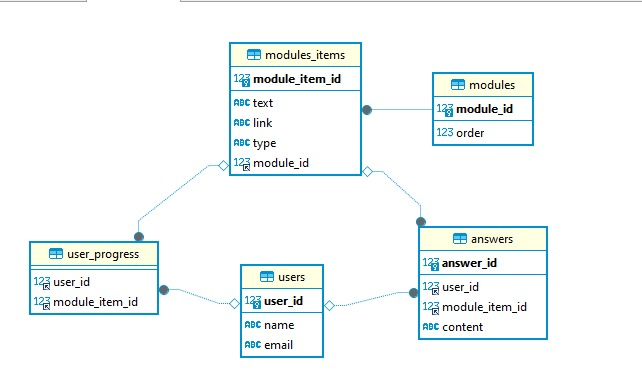
\includegraphics[width=1\linewidth]{conteudo//4 - ages III//conteudo//figures//bd.jpg}
        Fonte: https://tools.ages.pucrs.br/treinamentoAutoguiado/wiki/-/wikis/database
    \end{figure}

\subsection{Arquitetura Utilizada}
  Para disponibilizar a ferramenta, nós utilizamos a AWS\cite{aws}, que é um serviço cloud de fácil uso. Para fazer a instanciação dos recursos a serem utilizados foi usada a ferramenta Terraform, que permite fazer a definição de Infrastructure as Code, permitindo ver a arquitetura de forma mais clara e bem definida.

Inicialmente haviamos planejado uma arquitetura mais robusta, utilizando diversos serviços, porém, limitações foram impostas pela \ac{ages} e tivemos que simplificar o projeto, logo, acabamos utilizando uma EC2 para fazer o hosting tanto do backend e banco de dados, quanto do frontend e, também, para executar nossas pipelines com o GitLab Runner.

Por consequencia dessa escolha, a aplicação ficou com uma capacidade de usuários menor, dado que estava tendo que dividir poder computacional e espaço de armazenamento entre diversas aplicações. Além disso, não conseguimos criar um endereço customizado para a máquina, sendo necessário utilizar o endereço de IP público pré definido.

    \begin{itemize}
      \item https://tools.ages.pucrs.br/treinamentoAutoguiado/wiki/-/wikis/arquitetura
    \end{itemize}

    \begin{figure}[H]
        \centering
        \small
        \caption{Esquema de Recursos AWS Programa Manejos de Estresse}
        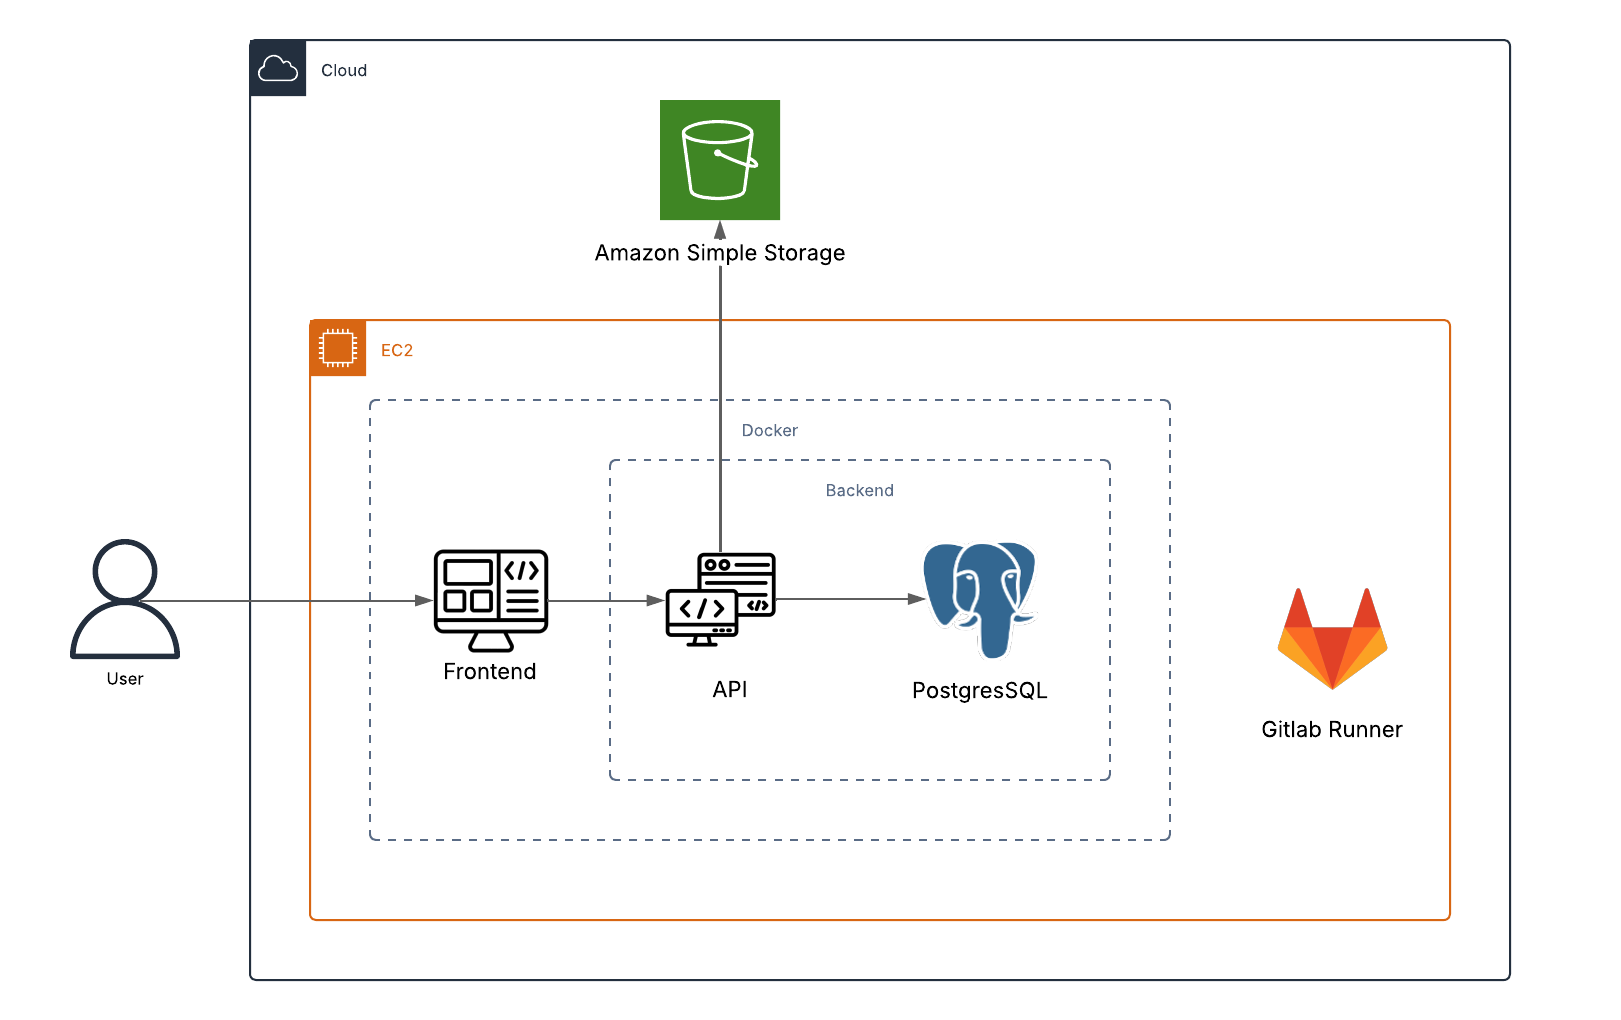
\includegraphics[width=1\linewidth]{conteudo//4 - ages III//conteudo//figures//arquitetura-aws.png}
        Fonte: https://tools.ages.pucrs.br/treinamentoAutoguiado/wiki/-/wikis/arquitetura
    \end{figure}

\subsection{Protótipos das Telas Desenvolvidas}
  Diferentemente das minhas duas primeiras AGES, nesse time, não possíamos um integrante que tivesse grande afinidade com Figma e um conhecimento amplo de design, somando isso ao fato de que precisavamos desenvolver uma plataforma web responsiva, tarefas desafiadoras foram apresentadas à equipe acerca do design, porém, acabamos conseguindo atingir um resultado que nos deixou bastante satisfeitos, fazendo utilização do design pattern utilizado na empresa das stakeholders e tentando seguir padrões de estilização mais amigáveis dada a natureza e o objetivo da plataforma.

    \begin{itemize}
      \item https://tools.ages.pucrs.br/treinamentoAutoguiado/wiki/-/tree/main TODO
    \end{itemize}

\subsection{Tecnologias Utilizadas}
  Para o desenvolvimento do projeto, foram utilizadas duas linguagens com diferentes técnologias para cada uma. Para o frontend foi utilizado o Typescript com a ferramenta React para o desenvolvimento e o Tailwind CSS para a estilização. Para o Backend optamos por utilizar a linguagem Java com o framework Sprintboot por serem amplamente conhecidas e de fácil uso, apesar da necessidade de fazer uma grande quantidade de boilerplate. Para o banco de dados foi escolhido o PostgreSQL por ser uma ferramenta de banco de dados relacional e de fácil uso, além de ser conhecida por diversos membros da equipe. Além das técnologias citadas, também foi utilizado o Docker para facilitar o desenvolvimento da aplicação, no qual executamos tanto o nosso banco de dados quanto nossa API dentro de um container, permitindo a fácil inicialização do projeto e que o mesmo fosse sempre executado sob as mesmas condições de configuração.

    \begin{itemize}
      \item https://tools.ages.pucrs.br/treinamentoAutoguiado/wiki/-/wikis/arquitetura
    \end{itemize}
